\documentclass[11pt]{article}

\usepackage[utf8]{inputenc}
\usepackage[spanish]{babel}
\usepackage{a4wide}
\usepackage{graphicx}
\usepackage{minted}

\title{Métodos Numéricos I - Resonancia en oscilaciones no lineales}
\author{Unai Aguilera Irazabal\\ DNI: 45663055M}

\begin{document}
\maketitle
\tableofcontents

\pagebreak
\renewcommand{\tablename}{Tabla}

\section{Introducción}
La ecuación diferencial (\ref{ecuacion-diferencial}) modela el comportamiento de
un oscilador no lineal en su forma más general.

\begin{equation}
\label{ecuacion-diferencial}
	 \frac{d^2 x}{dt^2} + \gamma\frac{dx}{dt} + \omega_{o}^2x 
	 + \beta{}x^2 = F_{o}\cos{\omega{}t}
\end{equation}

El primer término del lado izquierdo de esta ecuación representa la aceleración
que sufre el oscilador durante su movimiento. El segundo término define el 
amortiguamento del oscilador debido a la disipación de energía cinética mediante,
por ejempo, rozamiento. Dicho término es, por lo tanto, proporcional a la
velocidad del oscilador en cada instante y está regulado por el coeficiente
$\gamma$.

El tercer miembro es la fuerza lineal característica de los osciladores armónicos,
muelle, péndulo, etc. Este termino es proporcional a la frecuencia natural del
oscilador, $\omega_{o}$, determinada por sus características físicas: masa,
longitud del péndulo, constante elástica del muelle, etc.

El último termino del primer miembro de la ecucación introduce las 
características no lineales del oscilador mediante la aplicación de fuerzas que
dependen del cuadrado de la posición del oscilador en cada instante. Este
termino se encuentra regulado por el coeficiente $\beta$.

Por último, el miembro derecho de la ecuación representa la aplicación de una
fuerza externa sobre el oscilador. Esta fuerza posee una magnitud $F_{o}$ que
varía en el tiempo de forma periódica con una frecuencia $w$.

\section{Resolución numérica}
En esta sección se explican los aspectos relaciones con los métodos numéricos
utilizados en este trabajo para la resolución de los distintos casos del
oscilador anarmónico.

\subsection{Método de Runge-Kutta}
Para la resolución de la ecuación diferencial no lineal planteada en el trabajo,
se requiere la aplicación de un método númerico para la integración de
ecuaciones diferenciales. Este tipo de métodos permite obtener una solución
numérica en aquellos casos en los que no es posible llevar a cabo la resolución
de la ecuación diferencial por métodos analíticos. 

La obtención de la solución númerica de una ecuación diferencial se basa en la
aproximación del siguiente valor de la función mediante incrementos muy pequeños
de la variable independiente, utilizando para ello la información proporcionada
por la derivada de la función. La derivada es evaluada en cada paso,
obteniéndose la nueva razón del incremento de la variable dependiente para el
siguiente. Se obtiene así una tabla que contiene los valores de la función para
determinados valores. Normalmente, los valores de la variable independiente se
encuentran esquiespaciados entre sí debido a la utilización de un paso de
integración constante.

Como el enunciado del trabajo requiere la aplicación de un método numérico de
cuarto orden, se ha utilizado el método \textit{Runge-Kutta} de dicho orden
\footnote{página 460 del libro de Gerald \& Wheatley \textit{Análisis numérico
con aplicaciones}.}. En el método de Runge-Kutta, aplicado a la resolución de
una ecuación diferencial del tipo $\frac{dy}{dx}$, el incremento en $y$ no es
proporcional unicamente al valor de la derivada en el punto anterior, sino a un
promedio ponderado de varias estimaciones de dicho incremento. En el caso
concreto del método de cuarto orden utilizado, se obtiene un promedio ponderado
de cuatro estimaciones $k_n$ calculadas de forma incremental.

El método de Runge-Kutta de cuarto orden para la resolución de una ecuación
diferencial de primer grado queda definido por el siguiente conjunto de
ecuaciones:

\begin{equation}
	k_1 = hf(x_n, y_n)
\end{equation}

\begin{equation}
	k_2 = hf(x_n + \frac{1}{2}h, y_n + \frac{1}{2}k_1)
\end{equation}

\begin{equation}
	k_3 = hf(x_n + \frac{1}{2}h, y_n + \frac{1}{2}k_2)
\end{equation}

\begin{equation}
	k_4 = hf(x_n + h, y_n + k_3)
\end{equation} 

\begin{equation}
	y_{n+1} = y_{n} + \frac{1}{6}(k_1 + 2k_2 + 2k_3 + k_4)
\end{equation}

don del error se puede estimar como $O(h^5)$.

\subsubsection{Método de Runge-Kutta para ecuaciones diferenciales de segundo
grado}
\label{segundo_grado}
Para poder aplicar el método anterior a la resolución numérica de ecuaciones
diferenciales de segundo grado, como es el caso del oscilador anarmónico, es
necesario, primeramente, llevar a cabo una descomposición de la ecuación
planteada en un sistema de dos ecuaciones diferenciales de primer grado.
\footnote{páginas 477-478 del libro de Gerald \& Wheatley \textit{Análisis
numérico con aplicaciones}.}.

En el caso de la ecuación (\ref{ecuacion-diferencial}) del problema estudiado,
la realización de la substitución $\frac{dx}{dt} = y$, permite obtener el
siguiente sistema de ecuaciones:

\begin{equation}
	\frac{dx}{dt} = y = f(t, x, y)
\end{equation}

\begin{equation}
	\frac{dy}{dt} = F_{o}\cos{\omega{}t} -\gamma{}y - \omega_{o}^2x
	- \beta{}x^2 = g(t, x, y) 	
\end{equation}

donde se han indicado también las funciones $f(t, x, y)$ y $g(t, x, y)$ que se
utilizarán para la aproximación del sistema.

Por otro lado, el método de Runge-Kutta explicado anteriormente debe ser
modificado para poder ser aplicado al sistema de ecuaciones diferenciales de
forma correcta\footnote{página 480 del libro de Gerald \& Wheatley
\textit{Análisis numérico con aplicaciones}.}. 

En el metodo para un sistema de ecuaciones se alterna en la obtención de las
constantes $k_n, l_n$ para cada una de las ecuaciones. Además, se utilizan los
valores correspondientes a cada variable dependiente para el incremento durante
el cálculo de la siguiente constante. 

Así, el método de Runge-Kutta para el caso de un sistema de dos ecuaciones
diferenciales se define de la siguiente forma:

\begin{equation}
	k_1 = hf(t_n, x_n, y_n)
\end{equation}

\begin{equation}
	l_1 = hg(t_n, x_n, y_n)
\end{equation}

\begin{equation}
	k_2 = hf(t_n + \frac{1}{2}h, x_n + \frac{1}{2}k_1, y_n + \frac{1}{2}l_1)
\end{equation}

\begin{equation}
	l_2 = gf(t_n + \frac{1}{2}h, x_n + \frac{1}{2}k_1, y_n + \frac{1}{2}l_1)
\end{equation}

\begin{equation}
	k_3 = hf(t_n + \frac{1}{2}h, x_n + \frac{1}{2}k_2, y_n + \frac{1}{2}l_2)
\end{equation}

\begin{equation}
	k_3 = gf(t_n + \frac{1}{2}h, x_n + \frac{1}{2}k_2, y_n + \frac{1}{2}l_2)
\end{equation}

\begin{equation}
	k_4 = hf(t_n + h, x_n + k_3, y_n + l_3)
\end{equation}

\begin{equation}
	k_4 = hf(x_n + h, x_n + k_3, y_n + l_3)
\end{equation} 

\begin{equation}
	x_{n+1} = x_n + \frac{1}{6}(k_1 + 2k_2 + 2k_3 + k_4)
\end{equation}

\begin{equation}
	y_{n+1} = y_n + \frac{1}{6}(l_1 + 2l_2 + 2l_3 + l_4)
\end{equation}

\subsubsection{Estudio de la precisión del método de Runge-Kutta}
\label{precision-runge-kutta}
Se realiza a continuación un estudio de la precisión del metodo implementado
mediante la modificación del paso de integración $h$ y comparando los resultados
obtenidos para diferentes valores de $t$ de la función $x(t)$ hasta el octavo
decimal. 

El estudio de precisión se ha llevado a cabo aplicando el método las ecuaciones
definidas en la sección \ref{segundo_grado} con las condiciones iniciales
$x(0) = \frac{dx}{dt}(0) = 0$. En la tabla \ref{tab:precision} se recogen
resultados obtenidos cuando se reduce el paso de integración a la mitad. Como
puede observarse, los resultados mejoran hasta que convergen hasta siete
decimales cuando el paso de integración se cambia de $h = 0.01$ a $h=0.005$. 

La precisión de siete decimales es suficiente para llevar a cabo el estudio de
los diferentes casos del oscilador anarmónico. Debido a que se obtiene la misma
precisión para los dos valores de $h$, se ha seleccionado el mayor de los dos
con la finalidad de necesitar un menor número de iteraciones y reducir el tiempo
de cómputo y las necesidades de memoria. Por lo tanto, durante la realización de
los siguientes apartados de este trabajo, se utilizará $h = 0.01$ como paso de
integración de las diferentes ecuaciones diferenciales con la aplicación del
método de Runge-Kutta.  

\begin{table}[h]
\centering
\begin{tabular}{|c|c|c|c|c|c|}
\hline
t & $h = 0.08$ & $h = 0.04$ & $h = 0.02$ & $h = 0.01$ & $h = 0.005$ \\
\hline
0.00 & 0.00000000 & 0.00000000 & 0.00000000 & 0.00000000 & 0.00000000 \\ 
0.40 & 0.03729791 & 0.03729797 & 0.03729797 & 0.03729797 & 0.03729797 \\ 
0.80 & 0.12560652 & 0.12560665 & 0.12560666 & 0.12560666 & 0.12560666 \\ 
1.20 & 0.21776317 & 0.21776331 & 0.21776332 & 0.21776332 & 0.21776332 \\ 
1.60 & 0.26365461 & 0.26365463 & 0.26365463 & 0.26365463 & 0.26365463 \\ 
2.00 & 0.22867909 & 0.22867888 & 0.22867887 & 0.22867886 & 0.22867886 \\ 
2.40 & 0.10701479 & 0.10701434 & 0.10701431 & 0.10701431 & 0.10701431 \\ 
2.80 & -0.07889020 & -0.07889079 & -0.07889082 & -0.07889082 & -0.07889082 \\ 
3.20 & -0.29094257 & -0.29094316 & -0.29094319 & -0.29094320 & -0.29094320 \\ 
3.60 & -0.48987965 & -0.48988020 & -0.48988023 & -0.48988024 & -0.48988024 \\ 
4.00 & -0.64352628 & -0.64352678 & -0.64352682 & -0.64352682 & -0.64352682 \\ 
4.40 & -0.72838016 & -0.72838067 & -0.72838070 & -0.72838070 & -0.72838070 \\ 
4.80 & -0.72853695 & -0.72853749 & -0.72853753 & -0.72853753 & -0.72853753 \\ 
5.20 & -0.63596267 & -0.63596328 & -0.63596331 & -0.63596332 & -0.63596332 \\ 
5.60 & -0.45435681 & -0.45435747 & -0.45435751 & -0.45435751 & -0.45435751 \\ 
6.00 & -0.20634549 & -0.20634617 & -0.20634620 & -0.20634621 & -0.20634621 \\ 
\hline
\end{tabular}
\caption{Estudio de la precisión de la solución para distintos valores del paso
de integración $h$. Se han utilizado los parámetros $\gamma=0.52$, $\beta=1$,
$F_o = 0.516$ y $w=1.2$. La tabla muestra que los valores convergen hasta el
séptimo decimal en los casos en que $h = 0.01$ y $h=0.005$. Se ha representado
únicamente un periodo y se han muestreado valores cada $\Delta{t} = 0.4$ de la
tabla de integración obtenida tras la aplicación del método Runge-Kutta}
\label{tab:precision}
\end{table}

\subsection{Transformada de Fourier Discreta}
Para el cálculo del espectro de potencias de las distintas señales producidas
en cada uno de los casos del oscilador se ha aplicado la \textit{Transformada de
Fourier Discreta}. Este método de análisis matemático permite descomponer una
señal discreta, y periódica en el tiempo, en un conjunto de señales sinusoidales
constitutivas. Su finalidad es aproximar la señal periódica mediante una serie de
ondas sinusoidales de frecuencias definidas. Por otro lado, su uso implica que
se analiza un único periodo de la señal periódica mediante la obtención de una
muestra de $N$ valores.

La Transformada de Fourier Discreta aplicada a un conjunto de N valores $x(t)$,
dentro de un mismo periodo de la señal y medidos en instantes equiespaciados
donde $t = t_o + \Delta{t}$, se calcula como:

\begin{equation}
	F(k) = \sum\limits_{n=0}^{N-1} x(t) \exp(-i \frac{2\pi{}nk}{N}),~~~~~~~~~~
	n = 0, 1, 2, \ldots, N -1
\end{equation}

Como puede observarse, los resultados de la aplicación de esta ecuación a una
muestra de N puntos proporciona información sobre N frecuencias constitutivas, 
múltiplos $n = 0, 1, 2, \ldots, N -1$ de una frecuencia base.

Hay que tener en cuenta que este cálculo, tal y como ha sido implementado en
este trabajo, requiere $O(N^2)$ operaciones, por lo que para conjuntos de
muestra grandes el tiempo de operaciones a realizar puede resultar muy elevado.

En el caso de este trabajo, la implementación de la Transformada de Fourier
Discreta se ha llevado a cabo de forma directa, debido a que a durante la
realización del análisis espectral de las señales del oscilador se ha obtenido
un conjunto de 4 puntos por periodo, y posteriormente promediada sobre 50
periodos de la señal. Este número de operaciones puede ser procesadas en un
tiempo aceptable en un ordenador moderno. Sin embargo, en el caso de necesitar 
un numero grande muestras, es recomendable utilizar la \textit{Transformada
Rápida de Fourier}, que utiliza simetrías durante el cálculo de los coeficientes
de la señal para reducir enormemente el número de operaciones requeridas hasta
$O(N\log(N))$.

\section{Casos de estudio}
Se exponen a continuación los resultados obtenidos del estudio tanto de la señal
como del espectro de potencias para cada uno de los siguientes casos de la
ecuación \ref{ecuacion-diferencial}:

\begin{itemize}
\item Oscilador lineal no forzado ni amortiguado ($\gamma = \beta = F_o = 0$).
\item Oscilador lineal forzado pero no amortiguado ($\gamma = \beta = 0$ pero $F_o \neq 0$).
\item Oscilador lineal forzado y amortiguado ($\beta = 0$ pero $\gamma \neq 0, F_o \neq0$).
\item Oscilador no lineal forzado y amortiguado ($\gamma \neq 0, \beta \neq 0, F_o \neq 0$).
\end{itemize}

Aunque los tres primeros casos pueden ser resueltos de forma analítica para
encontrar la solución exacta, se ha llevado a cabo la resolución numérica de los
diferentes casos para comprobar que los métodos implementados se comportan de la
forma esperada. Para el estudio de todos los casos anteriores se han considerado
las siguientes condiciones iniciales: 

\begin{equation}
	x(0) = \frac{dx}{dt}(0) = 0
\end{equation}

\subsection{Oscilador lineal no forzado ni amortiguado}
El sistema de ecuaciones diferenciales queda en este caso con la forma 

\begin{equation}
	\frac{dx}{dt} = y = f(t, x, y)
\end{equation}

\begin{equation}
	\frac{dy}{dt} = -w_o^2 y = g(t, x, y)
\end{equation}

En el caso de que se apliquen las condiciones iniciales consideradas, debido a
que el oscilador armónico se encuentra inicialmente en reposo y no actúa ninguna
fuerza sobre el mismo, no se producirá ningun cambio en su situación a lo largo
del tiempo. Por otro lado, ya que no existe ningún movimiento armónico del
oscilador las frecuencias constitutivas de la señal poseen un valor exactamente
cero. Ambos resultados se muestran en la figura \ref{fig:caso_lineal}.

\begin{figure}
\centering
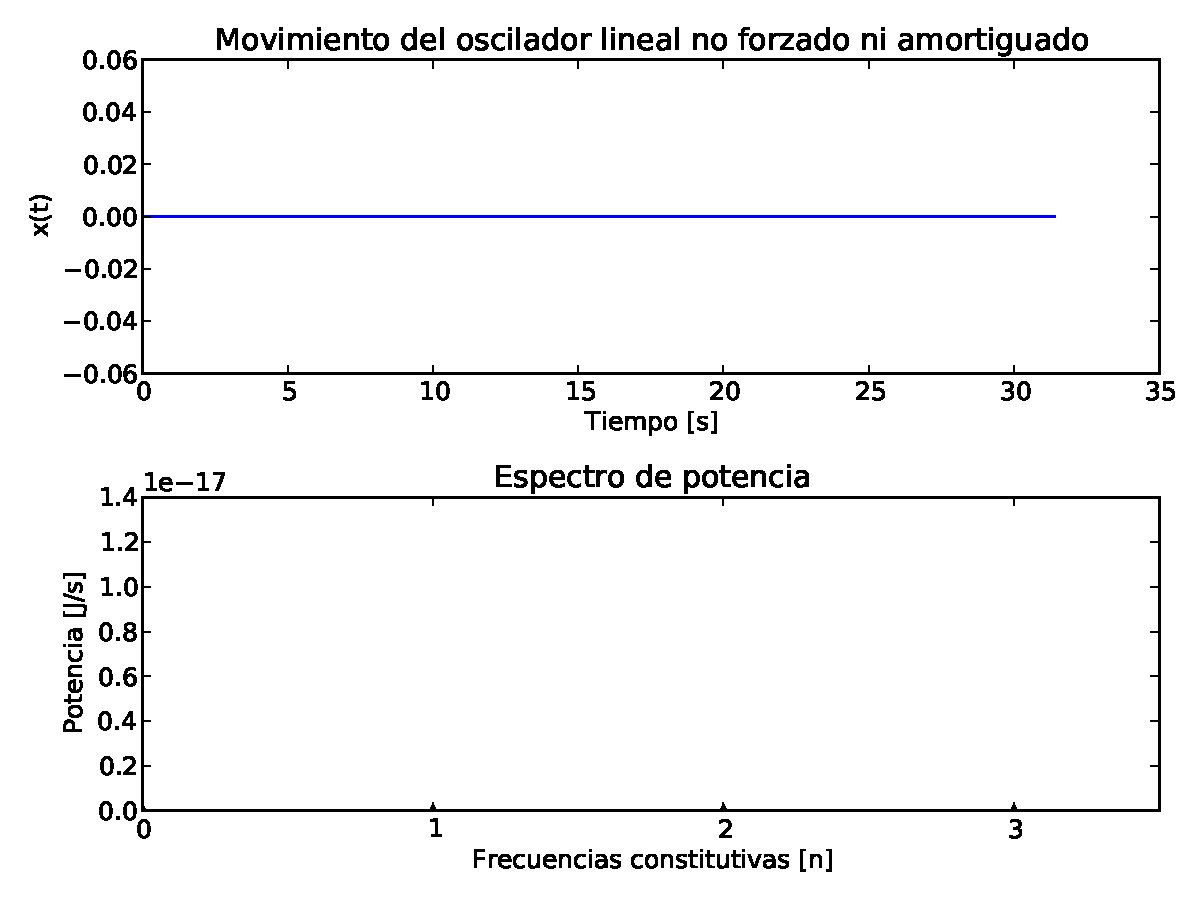
\includegraphics[width=0.75\linewidth]{caso_lineal.pdf}
\caption{Representación de la señal y espectro de potencias de un oscilador
lineal no forzado ni amortiguado con $w_o = 1$. La señal ha sido obtenida
mediante la aplicación del método de Runge-Kutta de cuarto orden y con un paso
de integración $h = 0.01$}
\label{fig:caso_lineal}
\end{figure}

\subsection{Oscilador lineal forzado pero no amortiguado}
Eliminando los términos cuyos coeficientes son cero en este caso
$(\gamma = \beta = F_o$, el sistema de ecuaciones tiene la siguiente forma

\begin{equation}
	\frac{dx}{dt} = y = f(t, x, y)
\end{equation}

\begin{equation}
	\frac{dy}{dt} = F_o\cos{wt} - w_o^2 x = g(t, x, y) 	
\end{equation}

donde se aplican las condiciones iniciales. 

El oscilador se encuentra en reposo y en el origen de coordendas, sin embargo,
la aplicación de la fuerza oscilante externa con una frecuencia igual a la
frecuencia natural del oscilador produce el fenómeno conocido como
\textit{resonancia}. Dicha fuerza externa proporciona energía al oscilador
aumentando la amplitud de su movimiento en cada ciclo, efecto que puede
observarse en la figura \ref{fig:caso_forzado}.

Por otro lado, en el espectro de potencias pueden observarse varias frecuencias
constitutivas que proporcionan, al sumar las componentes sinusoidales
correspondientes, la forma concreta de la señal. Hay que recordar, que una señal
sinusoidal pura y de extensión infinita estaría constituida por una única
componente de una frecuencia determinada. Sin embargo estas señal son teóricas y
no pueden representarse en un número finito de ciclos, por lo tanto, la señal
analizada tiene una longitud determinada en el tiempo y debe estar constituida
por varias frecuencias que sinteticen la forma adecuada.

\begin{figure}
\centering
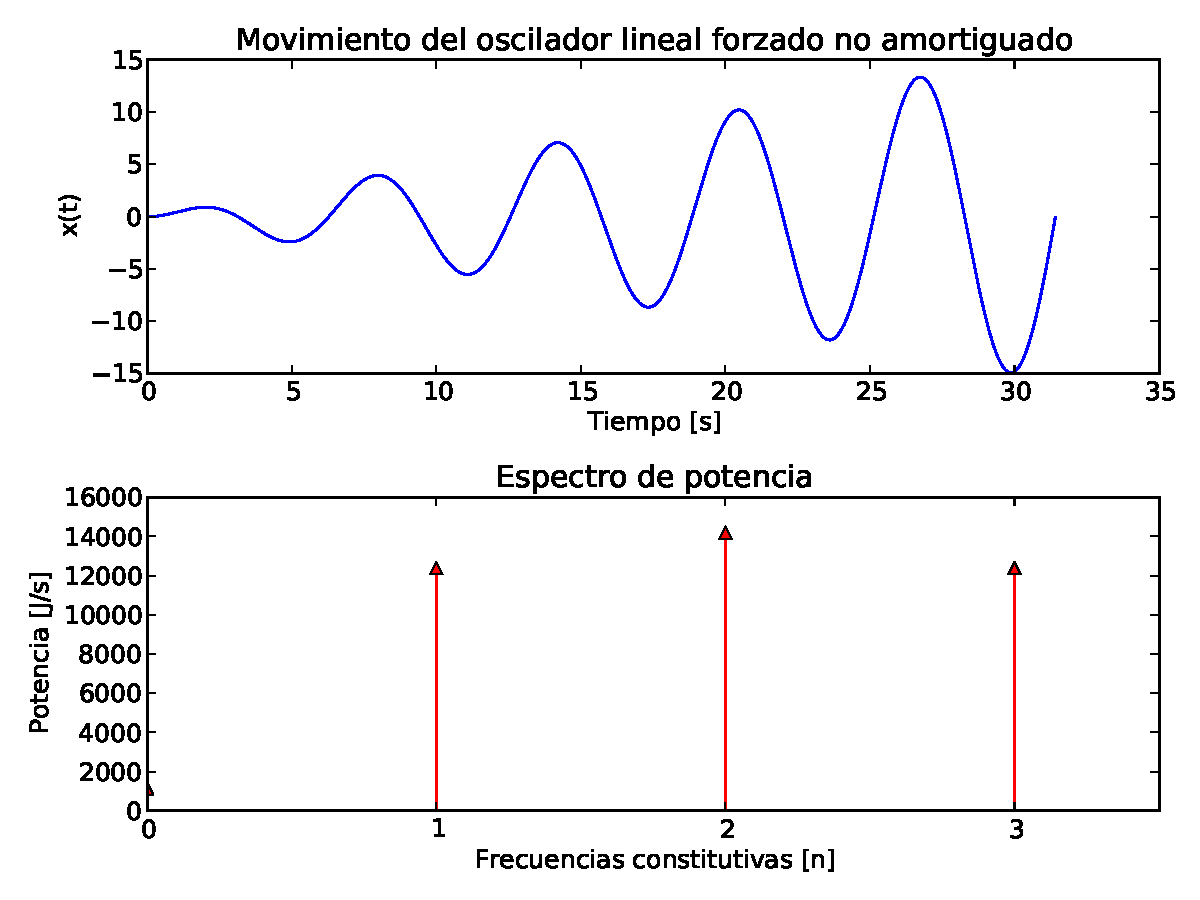
\includegraphics[width=0.75\linewidth]{caso_forzado.pdf}
\caption{Representación de la señal y del espectro de potencias de un oscilador
lineal forzado pero no amortiguado con $w_o = w = 1$ y un coeficiente para la
fuerza $F_o = 1$. La señal ha sido obtenida mediante la aplicación del método de
Runge-Kutta de cuarto orden y con un paso de integración $h = 0.01$.}
\label{fig:caso_forzado}
\end{figure}

\subsection{Oscilador lineal forzado y amortiguado}
En el caso de este tipo de oscilación se introduce un nuevo termino en el
sistema de ecuaciones que produce una disminución de la energía del oscilador
con el paso del tiempo.

\begin{equation}
	\frac{dx}{dt} = y = f(t, x, y)
\end{equation}

\begin{equation}
	\frac{dy}{dt} = F_o\cos{wt} - w_o^2 x - \gamma{}y = g(t, x, y) 	
\end{equation}

A partir de la aplicación de las condiciones iniciales y del método de
integración se obtiene la señal correspondiente al oscilador armónico forzado y
amortiguado. Como puede observarse en la figura\ref{fig:caso_forzado_amortiguado},
la amplitud del movimiento del oscilador no crece, como sí ocurre en el caso del
oscilador forzado y no amortiguado, de una forma indefinida debido a la 
aplicación de la fuerza periódica externa,

La introducción del factor de amortiguamiento, debido por ejemplo al rozamiento,
produce la reducción de la energía disponible. Sin embargo, ya que tanto la
fuerza periódica aplicada como la amortiguación son constantes en el tiempo, y
una vez que se termina la fase transitoria inicial, el oscilador produce una
señal sinusoidal de amplitud constante. Esto puede observarse al analizar el
espectro de frencuencias y comprobar que la forma del espectro es similar a la
del caso anterior. Sin embargo, en este caso la potencia de cada componente de
frecuencia es menor que el caso en el que no se produce amortiguación, debido a
que la amplitud de la señal se encuentra acotada.

\begin{figure}
\centering
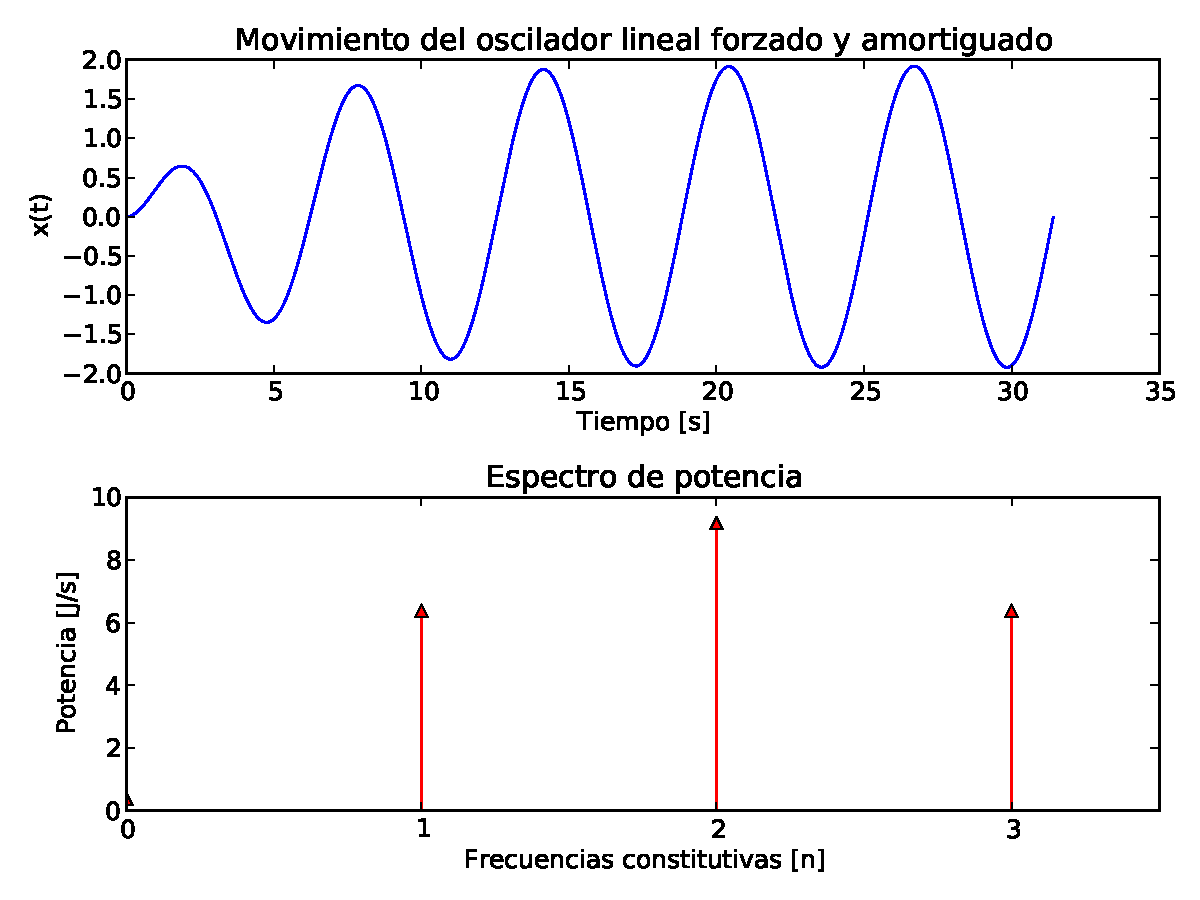
\includegraphics[width=0.75\linewidth]{caso_forzado_amortiguado.pdf}
\caption{Representación de la señal y del espectro de potencias de un oscilador
lineal forzado y amortiguado con $w_o = 1$, $w = 1$, $F_o = 1$ y un coeficiente
de amortiguamiento $\gamma = 0.52$. La señal ha sido obtenida mediante la
aplicación del método de Runge-Kutta de cuarto orden y con un paso de
integración $h = 0.01$}
\label{fig:caso_forzado_amortiguado}
\end{figure}

\subsection{Oscilador no lineal forzado y amortiguado}
En este último caso se utiliza la forma completa del sistema de ecuaciones
diferenciales que rige el movimiento del oscilador anarmónico:

\begin{equation}
	\frac{dx}{dt} = y = f(t, x, y)
\end{equation}

\begin{equation}
	\frac{dy}{dt} = F_{o}\cos{\omega{}t} -\gamma{}y - \omega_{o}^2x
	- \beta{}x^2 = g(t, x, y) 	
\end{equation}

y se utilizan nuevamente las condiciones iniciales y los métodos numéricos
correspondientes. En este caso se estudian dos conjuntos diferentes de
parámetros para el oscilador:

\begin{itemize}
	\item S1: $\gamma = 0.52$, $F_o = 0.516$, $w = 1.2$
	\item S2: $\gamma = 0.48$, $F_o = 0.5162$, $w = 1.3$
\end{itemize}

En ambos casos se ha utilizado $\beta=1.09$, con objeto de obtener un
comportamiento aperiódico claro en una representación en pocos periodos de la
señal.

\subsubsection{Conjunto de parámetros S1}
Al utilizar la configuración de parámetros dada y aplicar el método de
resolución de ecuaciones diferenciales de Runge-Kutta al sistema de ecuaciones
diferenciales se ha detectado el siguiente problema. La ecuación es inestable y
al llegar a cierto instante de tiempo se produce un estallido y un crecimiento
muy rápido que produce valores númericos no representables. En la figura
\ref{fig:caso_anarmonico_s1} se observa la representación obtenida hasta que se
produce el comportamiento inestable detectado. En esta situación es imposible
calcular un número suficiente de periodos que permita aplicar el análisis del
espectro de potencias llevado a cabo en los casos anteriores.

\begin{figure}
\centering
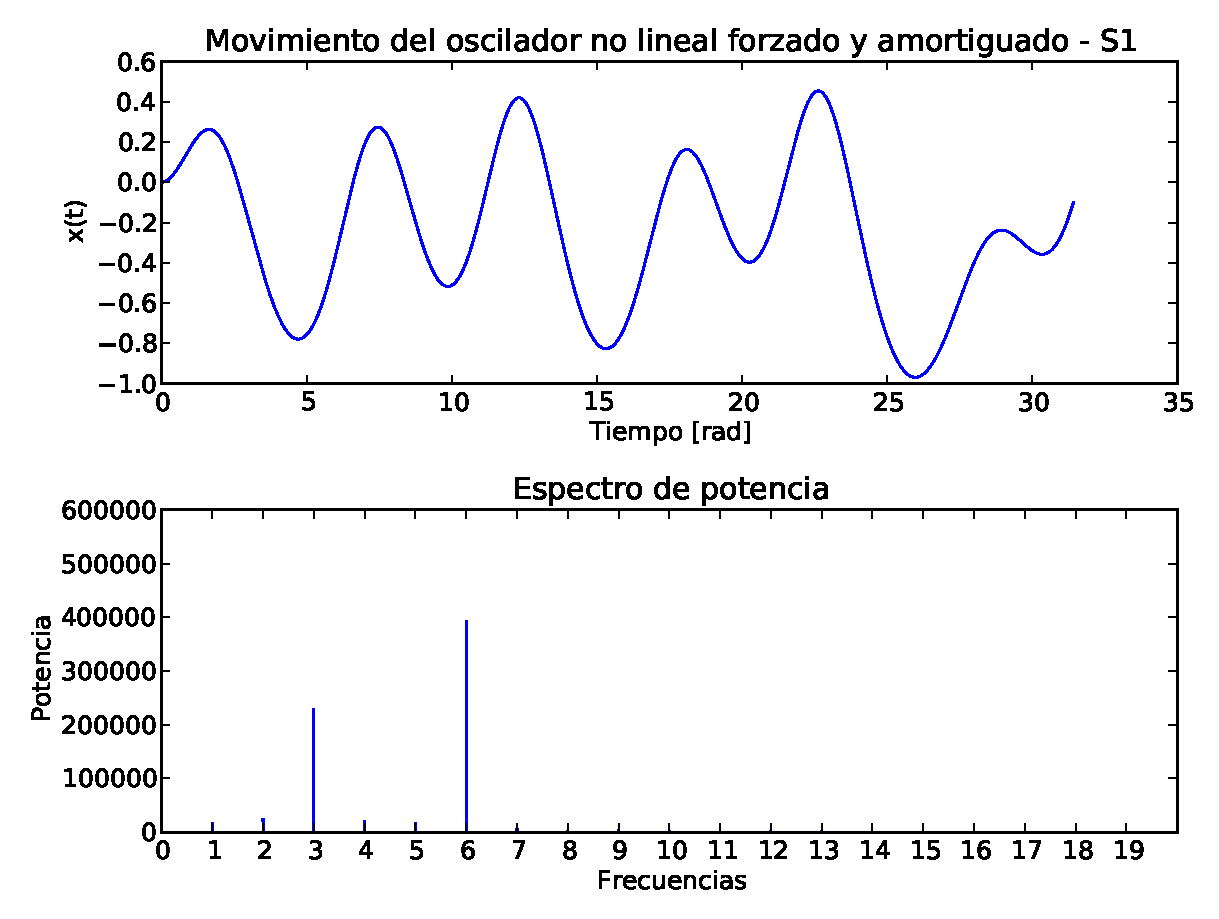
\includegraphics[width=0.75\linewidth]{caso_anarmonico_s1.pdf}
\caption{Representación de la señal y el espectro de potencias de un oscilador
anarmónico forzado y amortiguado con $w_o = 1$, $w = 1$, $\gamma = 0.52$,
$F_o = 0.516$, $w = 1.2$. La señal ha sido obtenida mediante la aplicación del
método de Runge-Kutta de cuarto orden y con un paso de integración $h = 0.01$}
\label{fig:caso_anarmonico_s1}
\end{figure}

La detección del comportamiento anómalo de la función se ha implementado
comprobando si en algún momento se obtiene un valor para $x(t)$ definido 
como NaN. Esto significa que la ecuación se ha vuelto inestable y ha comenzado 
a crecer en magnitud de forma descontrolada. Esta comprobación puede comprobarse
en los listados de código incluidos en el anexo del trabajo.

Con objeto de resolver el problema se ha probado a modificar el tamaño del paso
de integración, pero no se han obtenido resultados satisfactorios. La
inestabilidad en el sistema de ecuaciones se debe a la introducción del factor
no lineal en la ecuación y a su correspondiente coeficiente, que produce que
dicho término crezca de una forma mucho más rápida que los otros. Las
ecuaciones que contienen términos de este tipo se conocen como
\textit{ecuaciones rígidas} y presentan un comportamiento inestable ante ciertos
métodos númericos de integración

La solución al problema de la rigidez de las ecuaciones requiere la utilización
de otros métodos numéricos que produzcan un comportamiento más estable en las
ecuaciones integradas. Por ejemplo, se ha constatado en internet que existen
métodos como el \textit{Backward Euler Method}
\footnote{http://en.wikipedia.org/wiki/Backward\_Euler\_method } que pueden ser
aplicados a sistemas de ecuaciones diferenciales. Esta solución es similar al
método de Euler, pero utiliza un representación impĺícita de la función
diferencial y la construcción de un sistema de ecuaciones que debe ser resuelto
mediante algún metodo (p.e. el método de Newton o el del punto fijo). 

Sin embargo, el autor de este trabajo no ha conseguido representar correctamente
el sistema de ecuaciones diferenciales en una forma implícita para la aplicación
de este método.

\subsubsection{Conjunto de parámetros S2}
Al utilizar el segundo conjunto de parámetros ha sido posible calcular un número
de periodos suficiente como para llevar a cabo la integración de la señal
durante los periodos necesarios para realizar un análisis de frecuencia
promediado. El análisis de Fourier se ha llevado a cabo utilizando una
frecuencia de señal de $w=1.3$, es decir, igual a la frecuencia de la fuerza
periódica externa aplicada al oscilador.

En este caso puede observarse que aparece una nueva componente de frecuencia
$n=0$ y que es debida al comportamiento no periódico de la función de onda
analizada.

\begin{figure}
\centering
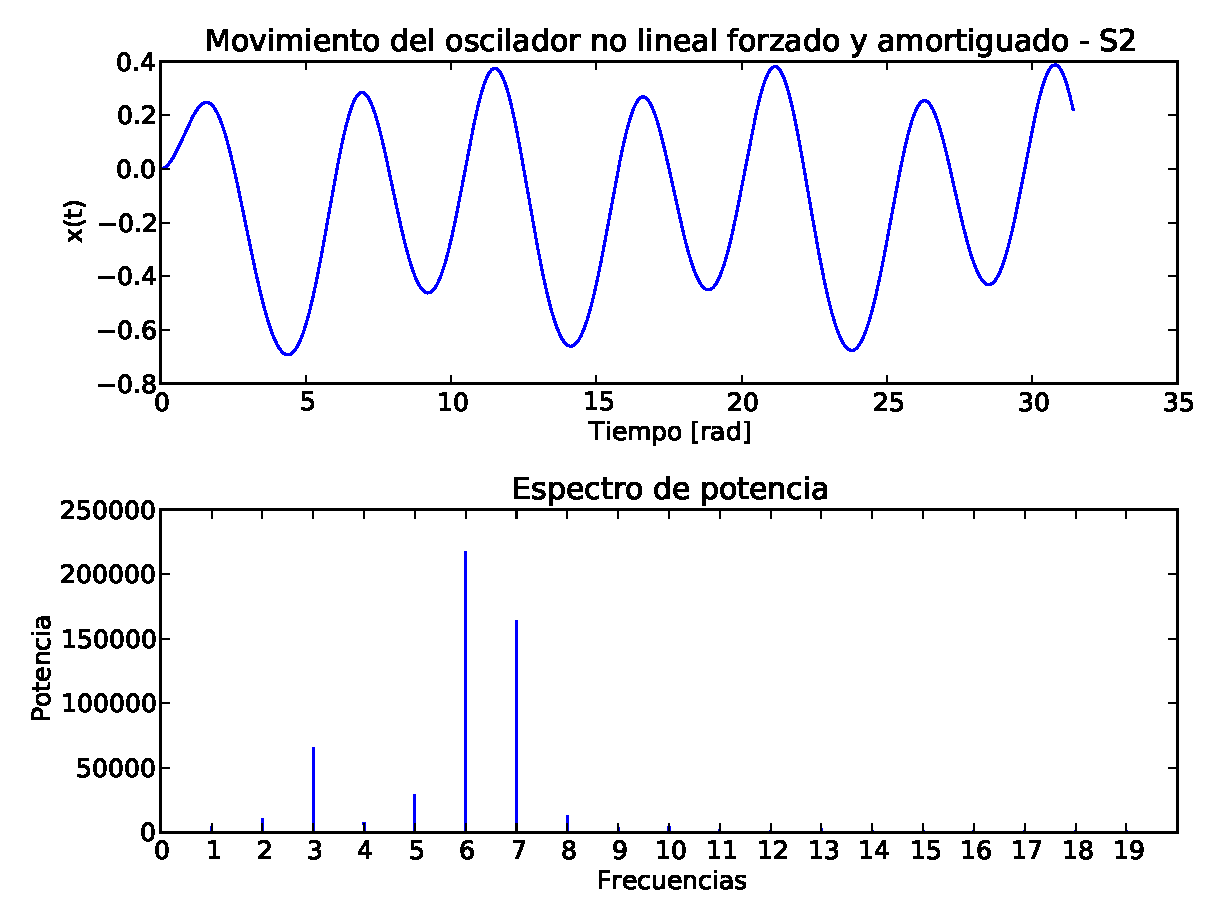
\includegraphics[width=0.75\linewidth]{caso_anarmonico_s2.pdf}
\caption{Representación de la señal y el espectro de potencias de un oscilador
anarmónico forzado y amortiguado con $w_o = 1$, $w = 1$, $\gamma = 0.48$,
$F_o = 0.5162$, $w = 1.3$. La señal ha sido obtenida mediante la aplicación del
método de Runge-Kutta de cuarto orden y con un paso de integración $h = 0.01$}
\label{fig:caso_anarmonico_s2}
\end{figure}

\section{Conclusiones}
La realización de este trabajo ha servido para comprobar el funcionamiento real
de un método de integración aplicado a un sistema de ecuaciones diferenciales.
Ha permitido comprobar cómo de importante es la elección del paso de integración
correcto para obtener la aproximación requerida de la aplicación del método
numérico.

Por otro lado, se ha conocido experimentalmente cuáles son las limitaciones de
los métodos de integración de tipo explícito, como es el caso del método de
Runge-Kutta utilizado, cuando se aplican a ecuaciones rígidas. Aunque no se ha
podido comprobar una implementación de un método implícito, se ha comprobado la
existencia de este tipo de métodos y su mayor adecuación para la resolución de
ecuaciones diferenciales en dichos casos.

Además, el trabajo ha permitido estudiar el funcionamiento de la Transformada de
Fourier Discreta y, mediante algunas pruebas realizadas durante la elaboración
del trabajo, comprobar que el incremento en el número de muestras de la señal
produce un aumento notable en el tiempo de computación de la misma. Aunque no se
ha llegado a implementar, se ha comprobado que la solución a este problema es la
utilización de la Transformada Rápida de Fourier mediante el uso de una
implementación de la misma proporcionada por la librería \textit{numpy} para
Python. Se ha comprobado que los resultados obtenidos con el uso de dicha
librería concuerdan con la implementación directa de la transformada discreta,
mientras que los tiempos de la Transformada Rápida de Fourier son muchísimo más
pequeños que los del código utilizado en el trabajo.

\section{Anexo}
\subsection{Implementación de los métodos numéricos}
La implementación de los diferentes métodos numéricos desarrollados en este trabajo
ha sido realizada utilizando el lenguaje de programación Python
(http://www.python.org/). La generación de las gráficas se ha llevado a cabo
usando la librería \textit{matplotlib} (http://matplotlib.org/) para este
lenguaje de programación. Se incluye a continuación un listado del código de los
diferentes métodos numéricos utilizados.

Para el desarrollo del código de la Transformada de Fourier Discreta y del
cálculo del espectro de potencias se utilizado la librería \textit{cmath}
\footnote{http://docs.python.org/2/library/cmath.html}, que proporciona
funciones matemáticas para su uso con números complejos. Aunque Python incorpora
soporte nativo para la aritmética de números complejos, la librería usual de
funciones matemáticas \textit{math}\footnote{http://docs.python.org/2/library/math.html}
no proporciona cálculos para este tipo de números.

\begin{figure}
\inputminted[linenos, firstline=22, lastline=66, fontsize=\footnotesize]{python}
{../metodos/eq_diferenciales.py}
\caption{Código de la implementación del método Runge-Kutta de cuarto orden para
la resolución de un sistema de de dos ecuaciones diferenciales}
\label{runge_kutta_code}
\end{figure}

\begin{figure}
\inputminted[linenos, firstline=1, lastline=41, fontsize=\footnotesize]{python}
{../metodos/transformada_fourier.py}
\caption{Código de la implementación de la Transformada de Fourier Discreta y el
muestreo de una señal sobre varios periodos}
\end{figure}

\begin{figure}
\inputminted[linenos, firstline=43, lastline=83, fontsize=\footnotesize]{python}
{../metodos/transformada_fourier.py}
\caption{Código de la Transformada de Fourier Discreta promedio y cálculo del
espectro de potencia}
\end{figure}

\begin{figure}
\inputminted[linenos, firstline=1, lastline=28, fontsize=\footnotesize]{python}
{../graficas.py}
\caption{Implementación del código para la visualización de la señal y el
espectro de potencia.
Se ha utilizado la librería matplotlib para la generación de las gráficas}
\end{figure}

\begin{figure}
\inputminted[linenos, firstline=29, lastline=61, firstnumber=29,
fontsize=\footnotesize] {python}{../graficas.py}
\caption{Continuación de la implementación del código para la visualización de
la señal y el espectro de potencia. Se ha utilizado la librería matplotlib para
la generación de las gráficas}
\end{figure}

\begin{figure}
\inputminted[linenos, fontsize=\footnotesize]{python}{../caso_forzado.py}
\caption{Código del caso lineal no amortiguado ni forzado}
\end{figure}

\begin{figure}
\inputminted[linenos, fontsize=\footnotesize]{python}{../caso_forzado.py}
\caption{Código del caso lineal forzado pero no amortiguado}
\end{figure}

\begin{figure}
\inputminted[linenos, fontsize=\footnotesize]{python}{../caso_forzado_amortiguado.py}
\caption{Código del caso lineal forzado y amortiguado}
\end{figure}

\begin{figure}
\inputminted[linenos, fontsize=\footnotesize]{python}
{../caso_anarmonico_forzado_amortiguado_s1.py}
\caption{Código del caso no lineal forzado y amortiguado para parámetros S1}
\end{figure}

\begin{figure}
\inputminted[linenos, fontsize=\footnotesize]{python}
{../caso_anarmonico_forzado_amortiguado_s2.py}
\caption{Código del caso no lineal forzado y amortiguado para parámetros S2}
\end{figure}

\end{document}